\documentclass[11pt,a4paper]{article}

% ------------------------------------------------------------------
%  EasySeva -- Human-Computer Interaction Report
% ------------------------------------------------------------------
\usepackage[utf8]{inputenc}
\usepackage[T1]{fontenc}
\usepackage[margin=1in]{geometry}
\usepackage{graphicx}
\usepackage{float}
\usepackage{xcolor}
\usepackage{amssymb}
\usepackage{booktabs}
\usepackage{longtable}
\usepackage{enumitem}
\usepackage{caption}
\usepackage{titlesec}
\usepackage{fancyhdr}
\usepackage[hidelinks]{hyperref}

\definecolor{navy}{HTML}{1B2B5C}
\definecolor{gov}{HTML}{1D4ED8}
\definecolor{teal}{HTML}{0F766E}
\definecolor{lightgray}{HTML}{F1F5F9}

\captionsetup{font=small,labelfont=bf,labelsep=period}
\setlist{itemsep=2pt,topsep=3pt}

\titleformat{\section}{\Large\bfseries\color{navy}}{\thesection}{0.6em}{}
\titleformat{\subsection}{\large\bfseries\color{navy}}{\thesubsection}{0.6em}{}
\titleformat{\subsubsection}{\normalsize\bfseries\color{gov}}{\thesubsubsection}{0.6em}{}

\pagestyle{fancy}
\fancyhf{}
\lhead{\small\color{navy}EasySeva}
\rhead{\small\color{navy}Human--Computer Interaction}
\cfoot{\thepage}
\renewcommand{\headrulewidth}{0.4pt}

% Figure helper: full-width screenshot with a caption.
\newcommand{\shot}[2]{%
  \begin{figure}[H]\centering%
  \fbox{\includegraphics[width=0.96\linewidth]{screenshots/#1}}%
  \caption{#2}\end{figure}}

% Principle item: \prin{Heuristic}{What it means}{How EasySeva applies it}
\newcommand{\prin}[3]{\item \textbf{#1.} \textit{#2} \\ #3}

\begin{document}

% ====================== TITLE PAGE ======================
\begin{titlepage}
\centering
\vspace*{1.2cm}
{\Huge\bfseries\color{navy} EasySeva\par}
\vspace{0.4cm}
{\LARGE Government Services, Made Easier\par}
\vspace{0.3cm}
{\large A Citizen-First Web Portal --- Human--Computer Interaction Design Report\par}
\vspace{1.6cm}

{\large\bfseries A Project Report submitted for the course\par}
\vspace{0.2cm}
{\Large\color{gov} Human--Computer Interaction\par}
\vspace{1.6cm}

\begin{tabular}{ll}
\multicolumn{2}{l}{\large\bfseries Submitted by:}\\[4pt]
Rohith Ganesh Kanchi & 23BCE5049 \\[3pt]
S D Madhumitha & 23BCE5058 \\[3pt]
S Azhagesh & 23BCE1205 \\
\end{tabular}

\vspace{1.4cm}
{\large\bfseries Faculty In-Charge\par}
\vspace{0.2cm}
{\large Dr.\ Kabilan K\par}

\vspace{1.4cm}
{\large Vellore Institute of Technology\par}

\vfill
\begin{tabular}{ll}
\textbf{Live application:} & \url{https://easyseva-rho.vercel.app} \\[3pt]
\textbf{Source repository:} & \url{https://github.com/rZk1809/easyseva} \\
\end{tabular}
\vspace{0.8cm}

\end{titlepage}

\tableofcontents
\newpage

% ====================== ABSTRACT ======================
\section{Abstract}
EasySeva is a responsive web portal that helps ordinary citizens \emph{discover},
\emph{apply for}, and \emph{track} government services --- with a Tamil Nadu
service context --- in their own language and at their own pace. The project was
built as a Human--Computer Interaction (HCI) prototype whose primary users are
first-time and low-digital-literacy citizens who often find official portals
intimidating, jargon-heavy, and error-prone.

This report explains what the application does, why it is useful, and --- in
depth --- how established HCI principles were deliberately applied on every
screen. We analyse the interface against four complementary frameworks: Jakob
Nielsen's ten usability heuristics, Ben Shneiderman's eight golden rules of
interface design, Don Norman's principles of interaction design, and the WCAG
POUR accessibility pillars. For each page of the application we provide a
screenshot, describe its purpose, and enumerate the specific principles used,
stating both \emph{what the principle means} and \emph{how it is realised in the
interface}. The report closes with a heuristic-coverage matrix and a reflection
on how good HCI directly improves the citizen's experience.

% ====================== INTRODUCTION ======================
\section{Introduction}

\subsection{What is EasySeva?}
Applying for a government document --- an income certificate, a scholarship, a
ration card, an old-age pension --- is a task almost every household faces.
Yet the digital experience is typically poor: dense forms with thirty fields on
one page, unexplained acronyms, English-only interfaces, no way to save progress,
and status updates that read like internal department codes. For a first-time or
less-confident user this is a wall.

EasySeva reimagines that experience around \emph{how citizens think} rather than
how departments are organised. It offers:
\begin{itemize}
  \item A catalogue of \textbf{nine services} across six citizen-centred
        categories (Certificates, Benefits, Education, Family, Senior Citizen,
        and Document Updates).
  \item A \textbf{guided, step-by-step} application flow --- eligibility check,
        document checklist, chunked form, review, and confirmation.
  \item \textbf{Passwordless OTP login}, \textbf{save-and-resume} drafts, and
        \textbf{application tracking} by reference number.
  \item A \textbf{trilingual} interface (English, Tamil, Hindi) and built-in
        \textbf{accessibility} controls (large text, high contrast, reduced
        motion).
\end{itemize}

\subsection{Who is it for, and why is it useful?}
The target users are citizens who are intimidated by bureaucracy: first-time
applicants, elderly users, and people with limited English or limited digital
experience. EasySeva is useful because it lowers every barrier that usually
causes abandonment or error: it speaks plain language, it shows exactly what is
needed before the user starts, it validates input as it is typed, it never loses
the user's work, and it explains every status in human terms. The result is that
a citizen can complete an application correctly \emph{the first time}, with
confidence and dignity.

\subsection{How HCI enables a good interaction}
Human--Computer Interaction is the study of designing systems around human
abilities, limitations, and expectations. A government portal is exactly the
kind of \emph{high-stakes, low-frequency, high-anxiety} task where good HCI
matters most: the user may use it once a year, cannot afford to make a mistake,
and has no training. By applying well-understood principles --- visibility of
status, error prevention, recognition over recall, user control, and universal
accessibility --- EasySeva turns an anxious, failure-prone chore into a calm,
predictable, and forgiving experience. The rest of this report demonstrates,
screen by screen, how each principle was applied.

% ====================== FRAMEWORKS ======================
\section{HCI Principles and Frameworks Used}
This section defines the frameworks referenced throughout the page-by-page
analysis.

\subsection{Nielsen's 10 Usability Heuristics}
\begin{enumerate}[label=N\arabic*.]
  \item \textbf{Visibility of system status} --- keep users informed through
        timely, appropriate feedback.
  \item \textbf{Match between the system and the real world} --- speak the
        users' language with familiar words and concepts.
  \item \textbf{User control and freedom} --- provide clearly marked exits,
        undo, and the freedom to change course.
  \item \textbf{Consistency and standards} --- follow platform and internal
        conventions so similar things look and behave similarly.
  \item \textbf{Error prevention} --- design to prevent problems before they
        occur, not just to report them.
  \item \textbf{Recognition rather than recall} --- make options, actions, and
        information visible so users need not remember things.
  \item \textbf{Flexibility and efficiency of use} --- allow both novices and
        experts to work in the way that suits them.
  \item \textbf{Aesthetic and minimalist design} --- show only what is relevant;
        remove clutter that competes for attention.
  \item \textbf{Help users recognise, diagnose, and recover from errors} ---
        express errors in plain language with a constructive next step.
  \item \textbf{Help and documentation} --- provide easy-to-search, task-focused
        help where it is needed.
\end{enumerate}

\subsection{Shneiderman's 8 Golden Rules}
\begin{enumerate}[label=S\arabic*.]
  \item Strive for consistency.
  \item Cater to universal usability (novices to experts, accessibility).
  \item Offer informative feedback.
  \item Design dialogs to yield closure.
  \item Prevent errors.
  \item Permit easy reversal of actions.
  \item Keep users in control (internal locus of control).
  \item Reduce short-term memory load.
\end{enumerate}

\subsection{Norman's Interaction Design Principles}
\begin{enumerate}[label=D\arabic*.]
  \item \textbf{Affordances and signifiers} --- controls look like what they do
        and signal how to use them.
  \item \textbf{Feedback} --- every action produces a perceivable result.
  \item \textbf{Mapping} --- the relationship between controls and effects is
        natural (e.g., a progress bar maps to steps completed).
  \item \textbf{Constraints} --- the design limits invalid actions.
  \item \textbf{Consistency} --- similar operations use similar elements.
  \item \textbf{Conceptual model} --- the interface helps users form a correct
        mental model of the process.
\end{enumerate}

\subsection{WCAG Accessibility Pillars (POUR)}
Content must be \textbf{Perceivable}, \textbf{Operable}, \textbf{Understandable},
and \textbf{Robust}. EasySeva addresses POUR through colour-contrast-aware
theming, full keyboard operability with visible focus, plain-language content,
and semantic, assistive-technology-friendly markup.

% ====================== DESIGN FOUNDATIONS ======================
\section{Design System and Foundations}
Before the page analysis, three cross-cutting foundations are worth noting
because they support \emph{consistency}, \emph{universal usability}, and
\emph{accessibility} on every screen.

\subsubsection{A consistent visual language (N4, S1, D5)}
All screens are built from a small set of reusable primitives --- Button, Card,
Input, Alert, Dialog, Badge, Progress --- driven by shared design tokens
(a navy/blue/teal palette, consistent radius and spacing scales, and a single
Inter typeface). This guarantees that a primary action, a status badge, or a
form field looks and behaves identically everywhere, so learning one screen
teaches the user every screen.

\subsubsection{Built-in accessibility controls (S2, POUR)}
Every page can be adapted by the user: three text sizes, a high-contrast theme,
and a reduced-motion mode that respects the operating-system preference. A
``skip to main content'' link, visible keyboard focus rings, 44--56 px touch
targets, and ARIA roles/labels are present throughout.

\subsubsection{Trilingual interface (N2, N7)}
The entire interface is available in English, Tamil, and Hindi. Language can be
chosen on the landing page or switched at any time from the header; the choice
is remembered across visits.

\shot{20-accessibility}{The Accessibility Settings page lets each user tune text
size, contrast, motion, and language --- an explicit realisation of
Shneiderman's rule to ``cater to universal usability.''}

\shot{21-high-contrast}{High-contrast mode (shown here together with the Tamil
interface). The dark, high-contrast theme improves perceivability for
low-vision users and demonstrates that the accessibility and language settings
apply globally and persist across pages.}

% ====================== PAGE BY PAGE ======================
\section{Page-by-Page HCI Analysis}
For each screen we state its \emph{purpose} and then enumerate the principles
applied, giving both the meaning of the principle and the concrete way it is
realised in the interface.

% ---- Landing ----
\subsection{Landing Page}
\shot{01-landing}{The landing page: a single clear value proposition, an
up-front language choice, and two obvious next actions.}
\textbf{Purpose.} Create trust in seconds and route the user to the one action
they came for --- start a service or track an existing one.
\begin{itemize}
  \prin{Aesthetic and minimalist design (N8)}{Show only what matters}{A
    single headline, one sub-line, the language choice, and exactly two buttons.
    There is no clutter competing for the first-time user's attention.}
  \prin{Match with the real world (N2)}{Use the user's language}{The promise
    ``Government services, made easier'' and ``Find, apply, and track \ldots in
    your language, at your pace'' is written the way a citizen thinks, not in
    departmental terminology.}
  \prin{Flexibility and efficiency (N7)}{Serve diverse users}{Language is chosen
    before anything else, so a Tamil- or Hindi-first user is never forced through
    an English wall (see Figure~\ref{fig:tamil}).}
  \prin{Recognition rather than recall (N6)}{Make choices visible}{The trust
    strip (Secure \& Private, 3 Languages, Save \& Resume, Step-by-Step) surfaces
    the system's key capabilities instead of expecting the user to discover them.}
  \prin{Affordance and signifiers (D1)}{Controls look actionable}{The solid
    ``Get Started'' button clearly affords the primary action; the secondary
    ``Track'' button is visually subordinate, mapping importance to appearance.}
\end{itemize}

\begin{figure}[H]\centering
\fbox{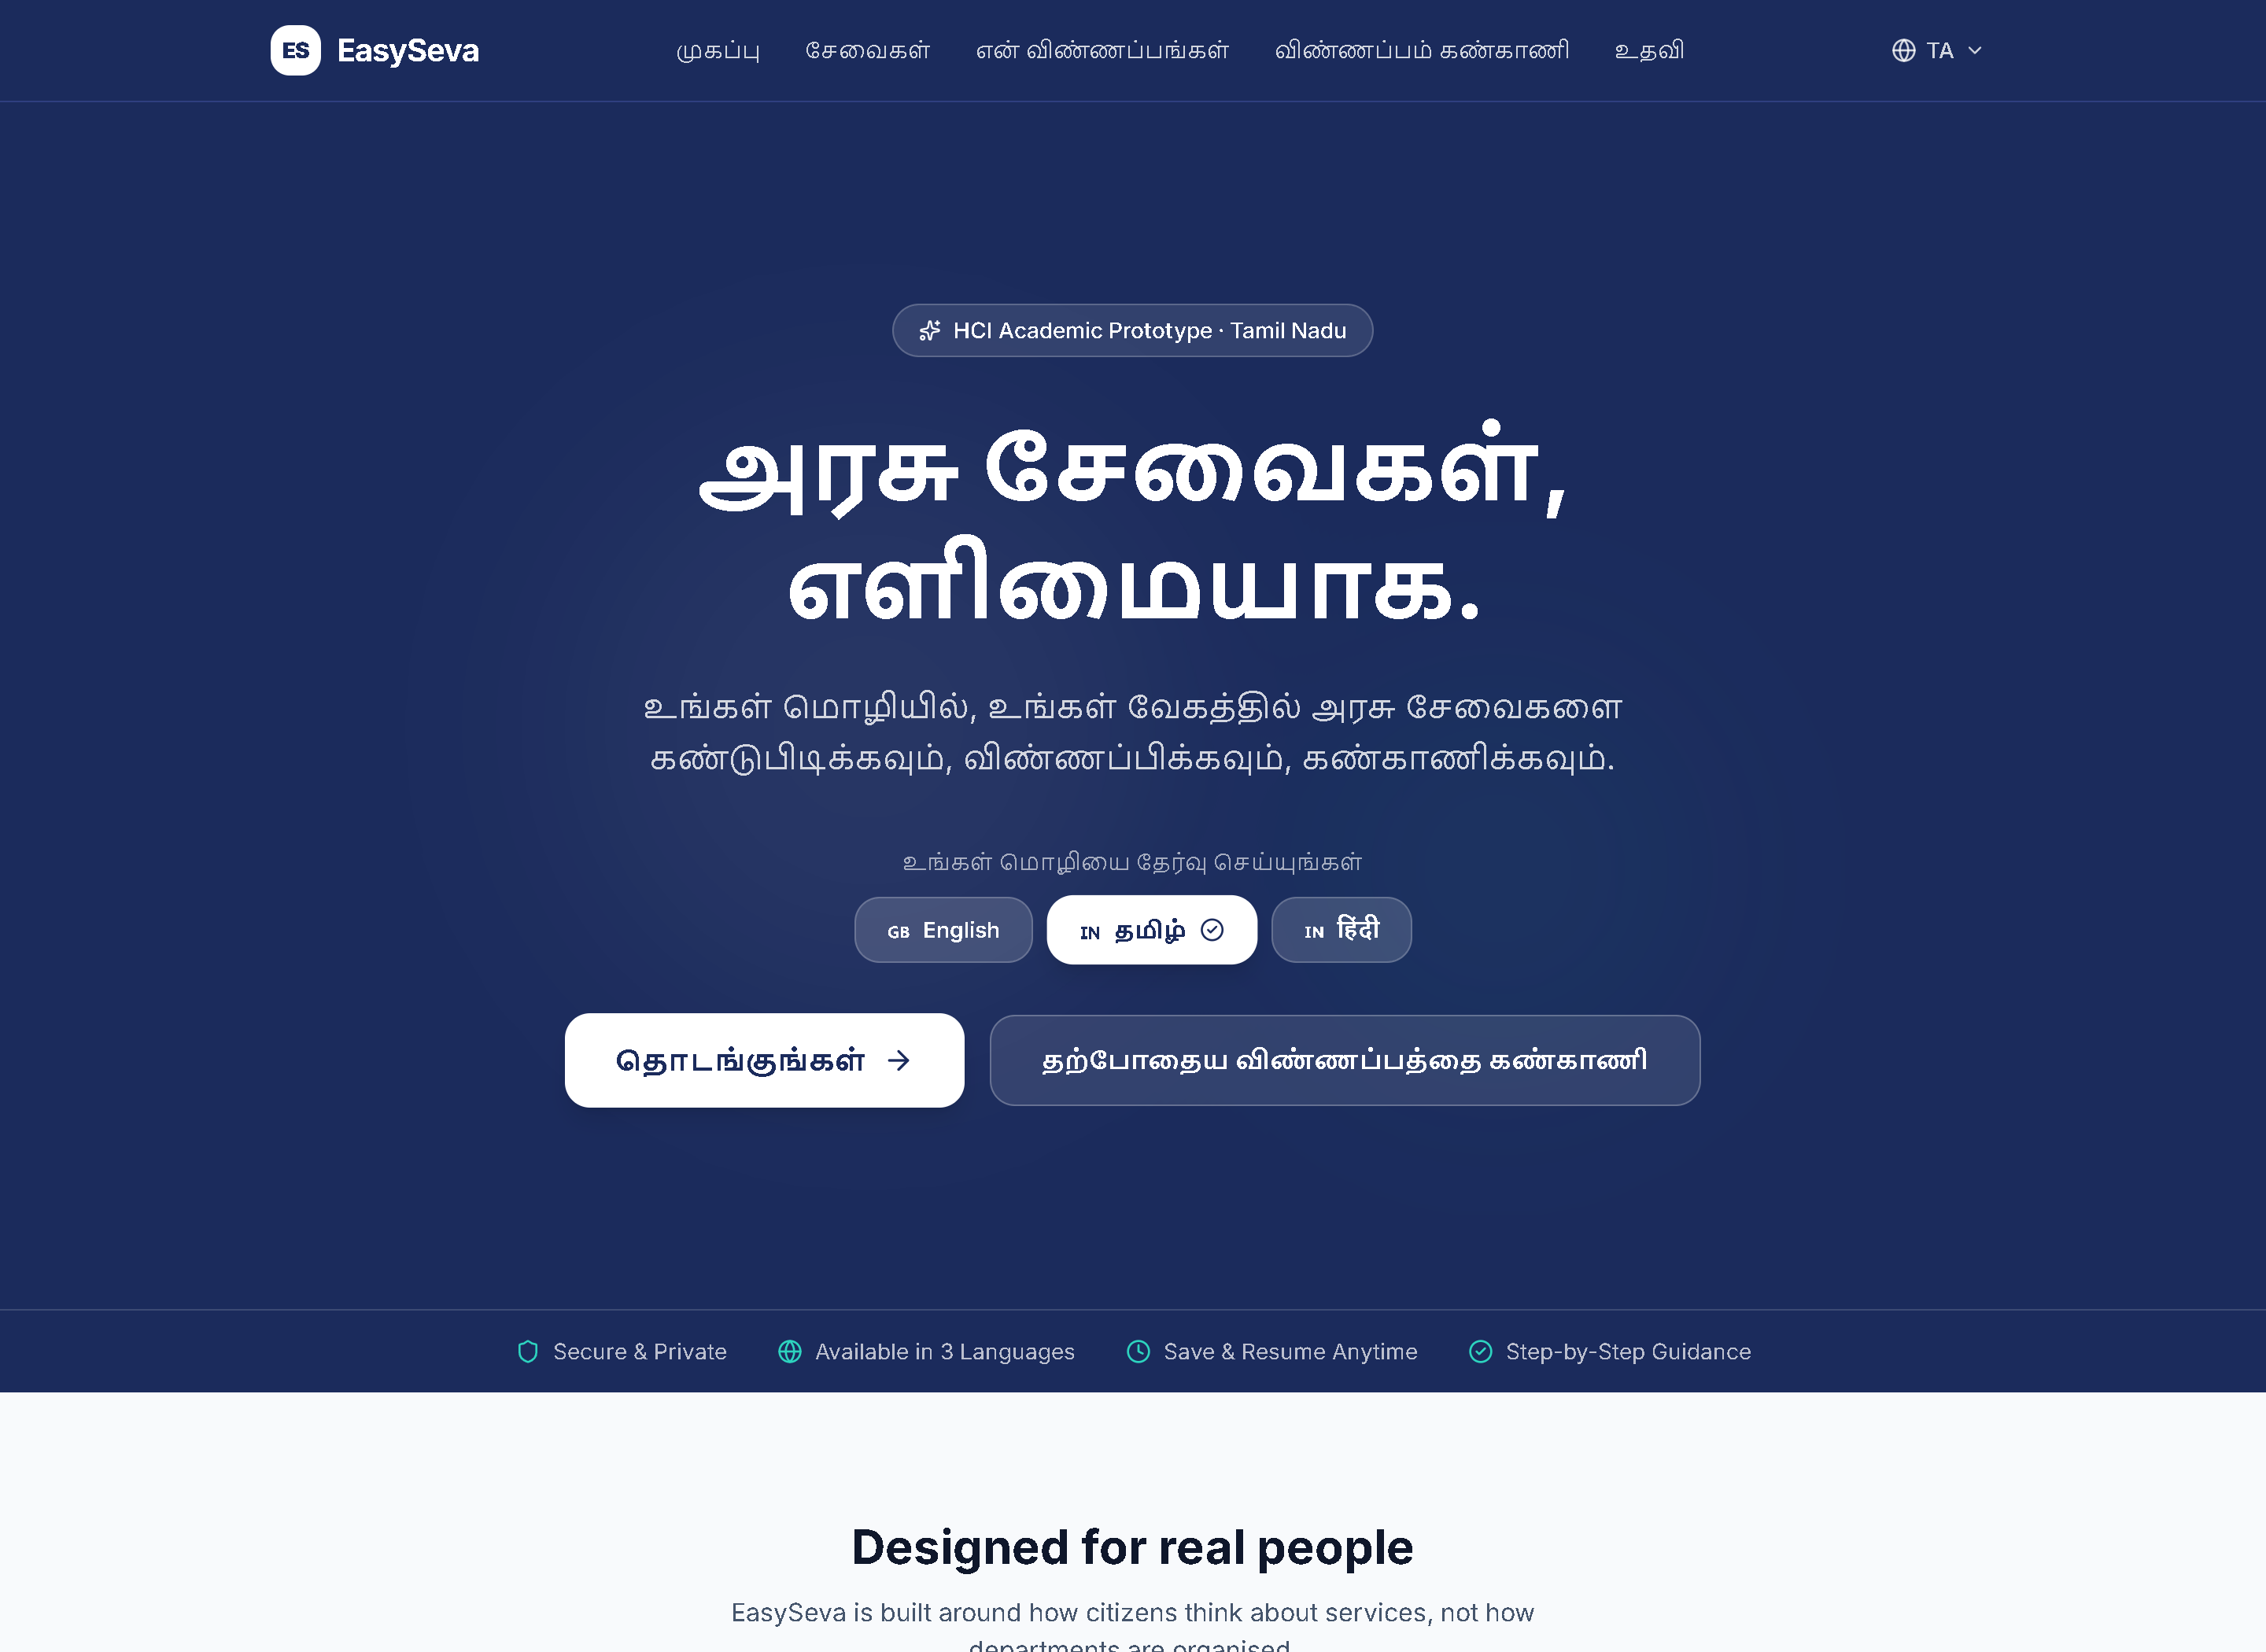
\includegraphics[width=0.96\linewidth]{screenshots/02-landing-tamil}}
\caption{The same landing experience in Tamil. Choosing a language rewrites the
entire interface, directly supporting ``match with the real world'' and
``flexibility of use'' for non-English speakers.}
\label{fig:tamil}
\end{figure}

% ---- Home ----
\subsection{Home Dashboard}
\shot{03-home}{The home dashboard: task-based service categories, a natural-
language search, a ``Help me find a service'' escape hatch, and the user's
recent applications with live status.}
\textbf{Purpose.} Give the signed-in citizen a single hub to begin a new task or
resume an existing one.
\begin{itemize}
  \prin{Match with the real world (N2)}{Organise by user goals}{Services are
    grouped as ``Get a Certificate,'' ``Find Government Benefits,'' ``Family
    Services'' --- citizen intents, not government department names.}
  \prin{Recognition rather than recall (N6)}{Show, don't make them remember}{Each
    category is a large card with an icon, title, and example services, so the
    user recognises the right path instead of recalling a menu.}
  \prin{Visibility of system status (N1, S3)}{Keep users informed}{The ``Recent
    Applications'' section shows each application's reference number and current
    status (e.g., ``Submitted'') so the user always knows where things stand.}
  \prin{Flexibility and efficiency (N7)}{Multiple routes}{Confident users can
    type a need into the search box; unsure users can click ``Help Me Find a
    Service'' to be guided by questions.}
\end{itemize}

% ---- Services + Category ----
\subsection{Service Catalogue and Category Pages}
\shot{04-services}{The full service catalogue, grouped into the six citizen-
centred categories with an accurate count of services in each.}
\shot{05-category}{A category page (Certificates) listing the services it
contains.}
\textbf{Purpose.} Let users browse the full catalogue or drill into a category.
\begin{itemize}
  \prin{Consistency and standards (N4, S1)}{Similar things look similar}{Every
    service and category is presented with the same card component, so browsing
    is predictable across the whole catalogue.}
  \prin{Recognition rather than recall (N6)}{Visible structure}{Category icons
    and short descriptions let users recognise where a service lives.}
  \prin{Aesthetic and minimalist design (N8)}{Reduce overload}{A large catalogue
    is chunked into six digestible groups rather than one long list.}
\end{itemize}

% ---- Service detail ----
\subsection{Service Detail Page}
\shot{06-service-detail}{The service detail page for Income Certificate:
breadcrumbs, a plain-language explanation, ``What you'll get,'' a document
checklist, a ``How it works'' overview, FAQs, and a Quick Information panel with
time, fee, processing duration, issuing department, and helpline.}
\textbf{Purpose.} Help the user decide, with confidence, whether and how to apply
--- \emph{before} committing time.
\begin{itemize}
  \prin{Help and documentation (N10)}{Task-focused help in place}{``What is this
    service?,'' ``You may need this for,'' and a dedicated FAQ accordion answer
    the citizen's real questions at the moment of decision.}
  \prin{Visibility of system status (N1)}{Set expectations}{The Quick Information
    panel states estimated time, fee, processing duration, the issuing
    department, and a helpline, so there are no surprises later.}
  \prin{Recognition rather than recall (N6)}{Orientation}{Breadcrumbs
    (Home / Services / Certificates / Income Certificate) always show where the
    user is and allow one-click return to any level.}
  \prin{Error prevention (N5, S5)}{Prepare before starting}{The ``Documents you
    will need'' checklist lets users gather everything \emph{before} they begin,
    preventing mid-form abandonment.}
  \prin{User control and freedom (N3, S7)}{No forced commitment}{A reassuring
    ``You can save and continue later'' note and a clear single primary action
    (``Start Application'') keep the user in control.}
\end{itemize}

% ---- Eligibility ----
\subsection{Eligibility Check}
\shot{07-eligibility}{The eligibility check asks one plain question at a time,
with an optional ``Why are we asking this?'' explanation and a progress bar.}
\shot{08-eligibility-result}{The result screen gives a clear verdict and --- even
when the user may not qualify --- preserves their freedom to continue or to find
a more suitable service.}
\textbf{Purpose.} Prevent wasted effort by checking suitability up front, without
discouraging the user.
\begin{itemize}
  \prin{Error prevention (N5, S5)}{Stop problems early}{Checking eligibility
    before the form prevents the larger ``filled everything, then rejected''
    failure.}
  \prin{Help and documentation (N10)}{Explain the ask}{Each question offers a
    ``Why are we asking this?'' disclosure, building understanding and trust.}
  \prin{Visibility of system status (N1, D3)}{Progress mapping}{A ``Question 1 of
    2'' progress bar maps directly to how far the user has come.}
  \prin{User control and freedom (N3, S7)}{Respect autonomy}{An ineligible result
    never blocks the user: they may ``Continue Anyway'' (an officer decides) or
    ask for help finding a different service.}
  \prin{Informative feedback (S3)}{Announce the outcome}{The result is wrapped in
    an \texttt{aria-live} region so screen-reader users hear the verdict
    immediately.}
\end{itemize}

% ---- Documents ----
\subsection{Document Upload}
\shot{09-documents}{The document step: each requirement is a self-contained card
with accepted formats, a size limit, examples of acceptable documents, and
upload or ``take photo'' actions.}
\textbf{Purpose.} Make uploading the right documents effortless and error-free.
\begin{itemize}
  \prin{Recognition rather than recall (N6)}{Show acceptable options}{A
    ``What can I use as \ldots?'' disclosure lists concrete examples (Aadhaar,
    Voter ID, \ldots) so the user need not recall what qualifies.}
  \prin{Error prevention (N5, S5)}{Validate before accepting}{Only PDF/JPG/PNG
    within the size limit are accepted; invalid files are rejected with a clear
    reason before any submission.}
  \prin{Visibility of system status (N1, S3)}{Confirm success}{An uploaded
    document turns green with a check and its file name and size, so the user
    sees it was accepted.}
  \prin{Flexibility and efficiency (N7)}{Fit the device}{Both ``Upload Document''
    and ``Take Photo'' are offered --- the latter is ideal on a phone.}
  \prin{Constraints (D4)}{Guide valid input}{The file picker is restricted to
    accepted file types, constraining the user toward a valid choice.}
\end{itemize}

% ---- Form ----
\subsection{Application Form}
\shot{10-form}{The form presents one small step at a time, with plain labels,
helper text, examples, and inline validation --- never a wall of thirty fields.}
\textbf{Purpose.} Collect accurate information with the least possible cognitive
load.
\begin{itemize}
  \prin{Reduce short-term memory load (S8, N6)}{Chunk the work}{The form is split
    into small, themed steps (Personal, Contact, Address, Income) instead of one
    overwhelming page.}
  \prin{Error prevention (N5, S5)}{Catch mistakes as they happen}{Fields validate
    inline (e.g., a 12-digit Aadhaar, a 10-digit mobile, a 6-digit PIN) with
    specific, friendly messages.}
  \prin{Match with the real world (N2)}{Human labels}{Labels and helper text use
    everyday phrasing (``Estimated Annual Income of Household'') with worked
    examples.}
  \prin{Visibility of system status (N1, D3)}{Show progress}{A step indicator
    shows how many steps remain, mapping effort to completion.}
  \prin{User control and freedom (N3, S6)}{Never lose work}{``Save \& Finish
    Later'' persists a draft at any point; users can leave and return safely.}
\end{itemize}

% ---- Review ----
\subsection{Review Before Submit}
\shot{11-review}{The review screen summarises every entered value and uploaded
document in collapsible sections, each independently editable, with a final
confirmation gate before submission.}
\textbf{Purpose.} Let the user verify everything and correct anything before the
irreversible submit.
\begin{itemize}
  \prin{Recognition rather than recall (N6)}{Summarise, don't quiz}{Every answer
    and document is shown back to the user, so they verify by recognition rather
    than trying to remember what they typed.}
  \prin{User control and freedom (N3, S6)}{Easy reversal}{An ``Edit'' control on
    each section jumps straight back to that part of the form.}
  \prin{Error prevention (N5, S5)}{Confirm before commit}{A warning banner and a
    confirmation dialog (``You cannot undo this action'') guard the final submit.}
  \prin{Design dialogs to yield closure (S4)}{Clear end of task}{The review marks
    a definite ``check, then submit'' close to the data-entry phase.}
\end{itemize}

% ---- Confirmation ----
\subsection{Confirmation}
\shot{12-confirmation}{The confirmation screen acknowledges success, shows the
reference number to save, and explains what happens next.}
\textbf{Purpose.} Reassure the user that their application was received and tell
them the next steps.
\begin{itemize}
  \prin{Visibility of system status (N1, S3)}{Unambiguous success}{A success
    state plus a prominent reference number confirms the submission landed.}
  \prin{Design dialogs to yield closure (S4)}{Complete the task}{The flow ends
    with a clear ``done'' state and a what-happens-next explanation, giving the
    user psychological closure.}
  \prin{Help users recover and plan (N10)}{Tell them what is next}{Guidance on
    tracking and expected timelines prevents the common ``what now?'' anxiety.}
\end{itemize}

% ---- Track ----
\subsection{Track an Application}
\shot{13-track}{Tracking by reference number --- available even without signing
in --- returns a plain-language status and timeline.}
\textbf{Purpose.} Let anyone check progress quickly, including users who applied
on someone's behalf.
\begin{itemize}
  \prin{Flexibility and efficiency (N7)}{Low-friction access}{Tracking works
    without login, so a family member can check status with just the reference
    number.}
  \prin{Match with the real world (N2)}{Plain status}{Statuses read as
    ``Officer Verification'' or ``Documents Verified,'' not internal codes.}
  \prin{Visibility of system status (N1)}{Progress at a glance}{A staged timeline
    shows exactly where the application is in the pipeline.}
\end{itemize}

% ---- Applications ----
\subsection{My Applications}
\shot{14-applications}{The applications list with Active / Drafts / Completed
tabs, search, and a status badge on every item.}
\textbf{Purpose.} A personal workspace to monitor and resume all applications.
\begin{itemize}
  \prin{Visibility of system status (N1, S3)}{Status everywhere}{Each item
    carries a colour-coded status badge for an at-a-glance overview.}
  \prin{Flexibility and efficiency (N7)}{Filter and find}{Tabs separate Active,
    Drafts, and Completed, and a search box finds items by name or reference.}
  \prin{Consistency and standards (N4, S1)}{Familiar patterns}{The same card and
    badge components used elsewhere reappear here, so nothing must be relearned.}
\end{itemize}

% ---- Notifications ----
\subsection{Notifications}
\shot{15-notifications}{Notifications keep the citizen informed of each application
events, with unread indicators and the ability to mark items read.}
\textbf{Purpose.} Proactively surface changes so the user is never left guessing.
\begin{itemize}
  \prin{Visibility of system status (N1, S3)}{Proactive feedback}{Status changes
    and required actions are pushed to the user rather than hidden.}
  \prin{User control and freedom (N3, S7)}{Manage the inbox}{Users can mark a
    single item or all items as read, staying in control of their feed.}
  \prin{Recognition rather than recall (N6)}{Unread cues}{An unread count on the
    header bell and per-item styling make new information obvious.}
\end{itemize}

% ---- Profile ----
\subsection{Profile}
\shot{16-profile}{The profile page lets users view and edit their contact
details with clear save feedback.}
\textbf{Purpose.} Give users ownership of their own account information.
\begin{itemize}
  \prin{User control and freedom (N3, S7)}{Own your data}{Users edit their name
    and phone number directly.}
  \prin{Informative feedback (S3, N1)}{Confirm the save}{Saving produces an
    explicit ``changes saved'' confirmation.}
  \prin{Error prevention (N5)}{Validate contact details}{Inputs are validated
    before they are accepted.}
\end{itemize}

% ---- Login + Verify ----
\subsection{Sign In (OTP) and Verification}
\shot{17-login}{Passwordless sign-in: the user enters only an email address.}
\shot{18-verify}{The verification screen with a six-box OTP input, a resend
control with cooldown, and (in demo mode) the code shown on screen.}
\textbf{Purpose.} Authenticate users with the least friction and the least chance
of being locked out.
\begin{itemize}
  \prin{Error prevention (N5, S5)}{Remove a failure mode}{A one-time code means
    there is no password to forget, reuse, or mistype.}
  \prin{Flexibility and efficiency (N7)}{Fast entry}{The six-digit code can be
    pasted and auto-distributes across the boxes; focus advances automatically.}
  \prin{Visibility of system status (N1, S3)}{Show every state}{``Sending OTP,''
    ``Verifying,'' and ``Verified'' states are shown explicitly.}
  \prin{Help users recover from errors (N9)}{Graceful recovery}{A wrong code
    clears the boxes with a clear message; ``Resend OTP'' has a visible cooldown
    so users are not left stranded.}
  \prin{Affordance (D1)}{Obvious input}{Six separate boxes afford a six-digit
    code and signal exactly how much to type.}
\end{itemize}

% ---- Help ----
\subsection{Help Centre}
\shot{19-help}{The Help page answers common questions in plain language.}
\textbf{Purpose.} Provide searchable, task-oriented support.
\begin{itemize}
  \prin{Help and documentation (N10)}{Findable answers}{Frequently asked
    questions are organised and phrased the way citizens ask them.}
  \prin{Match with the real world (N2)}{Plain answers}{Answers avoid jargon and
    describe actions in user terms.}
\end{itemize}

% ---- Mobile ----
\subsection{Responsive and Mobile Experience}
\begin{figure}[H]\centering
\fbox{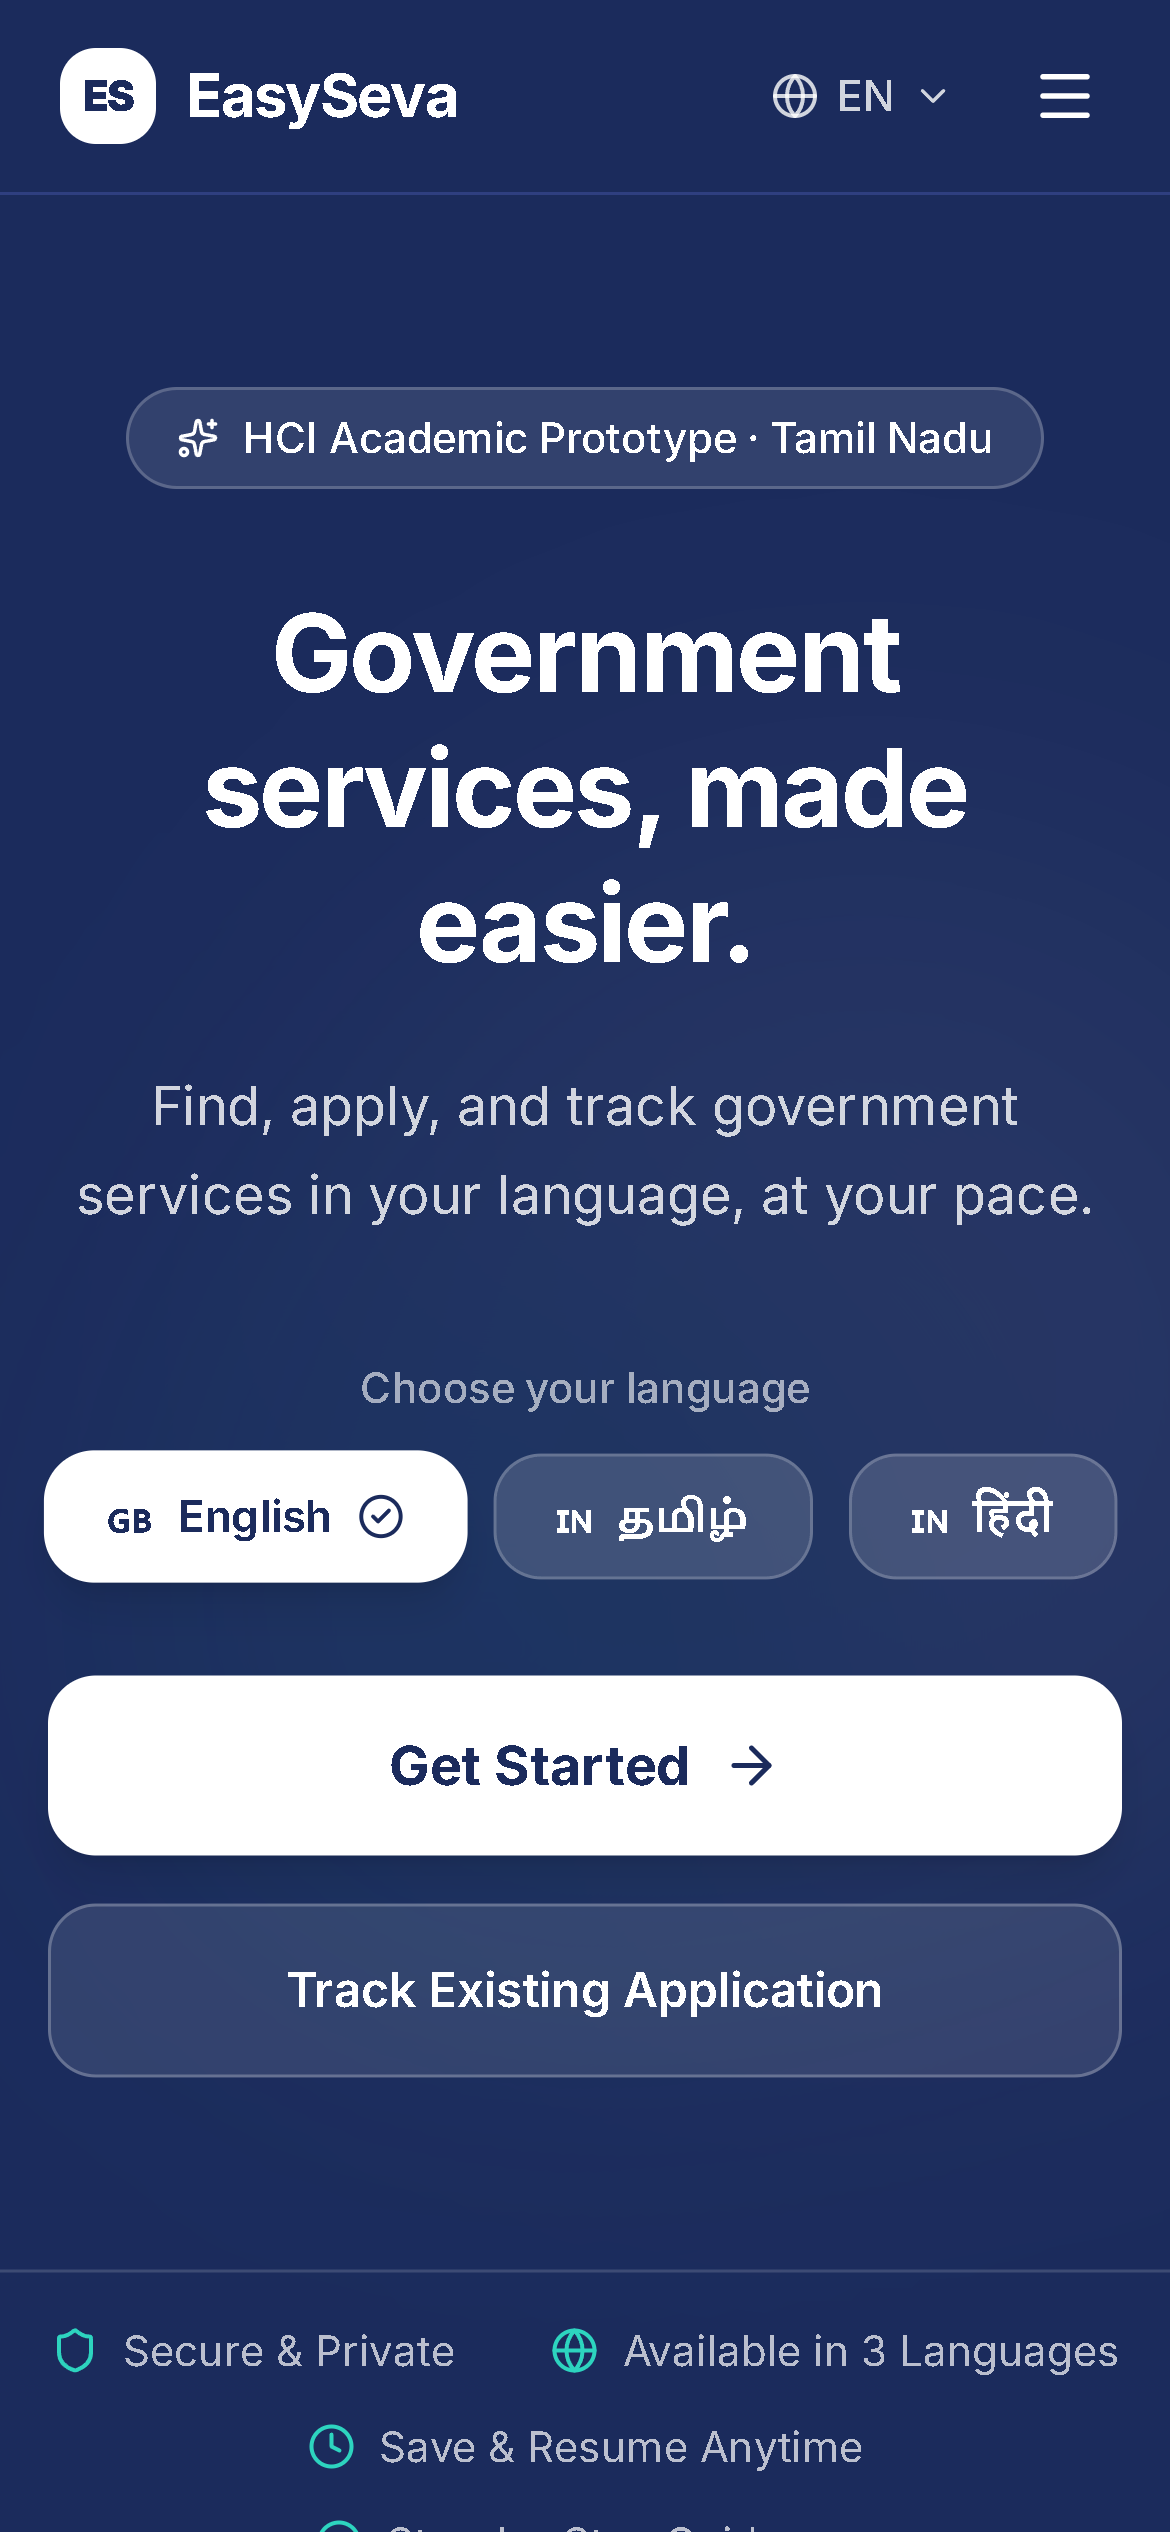
\includegraphics[height=9.5cm]{screenshots/22-mobile-landing}}\hspace{0.5cm}
\fbox{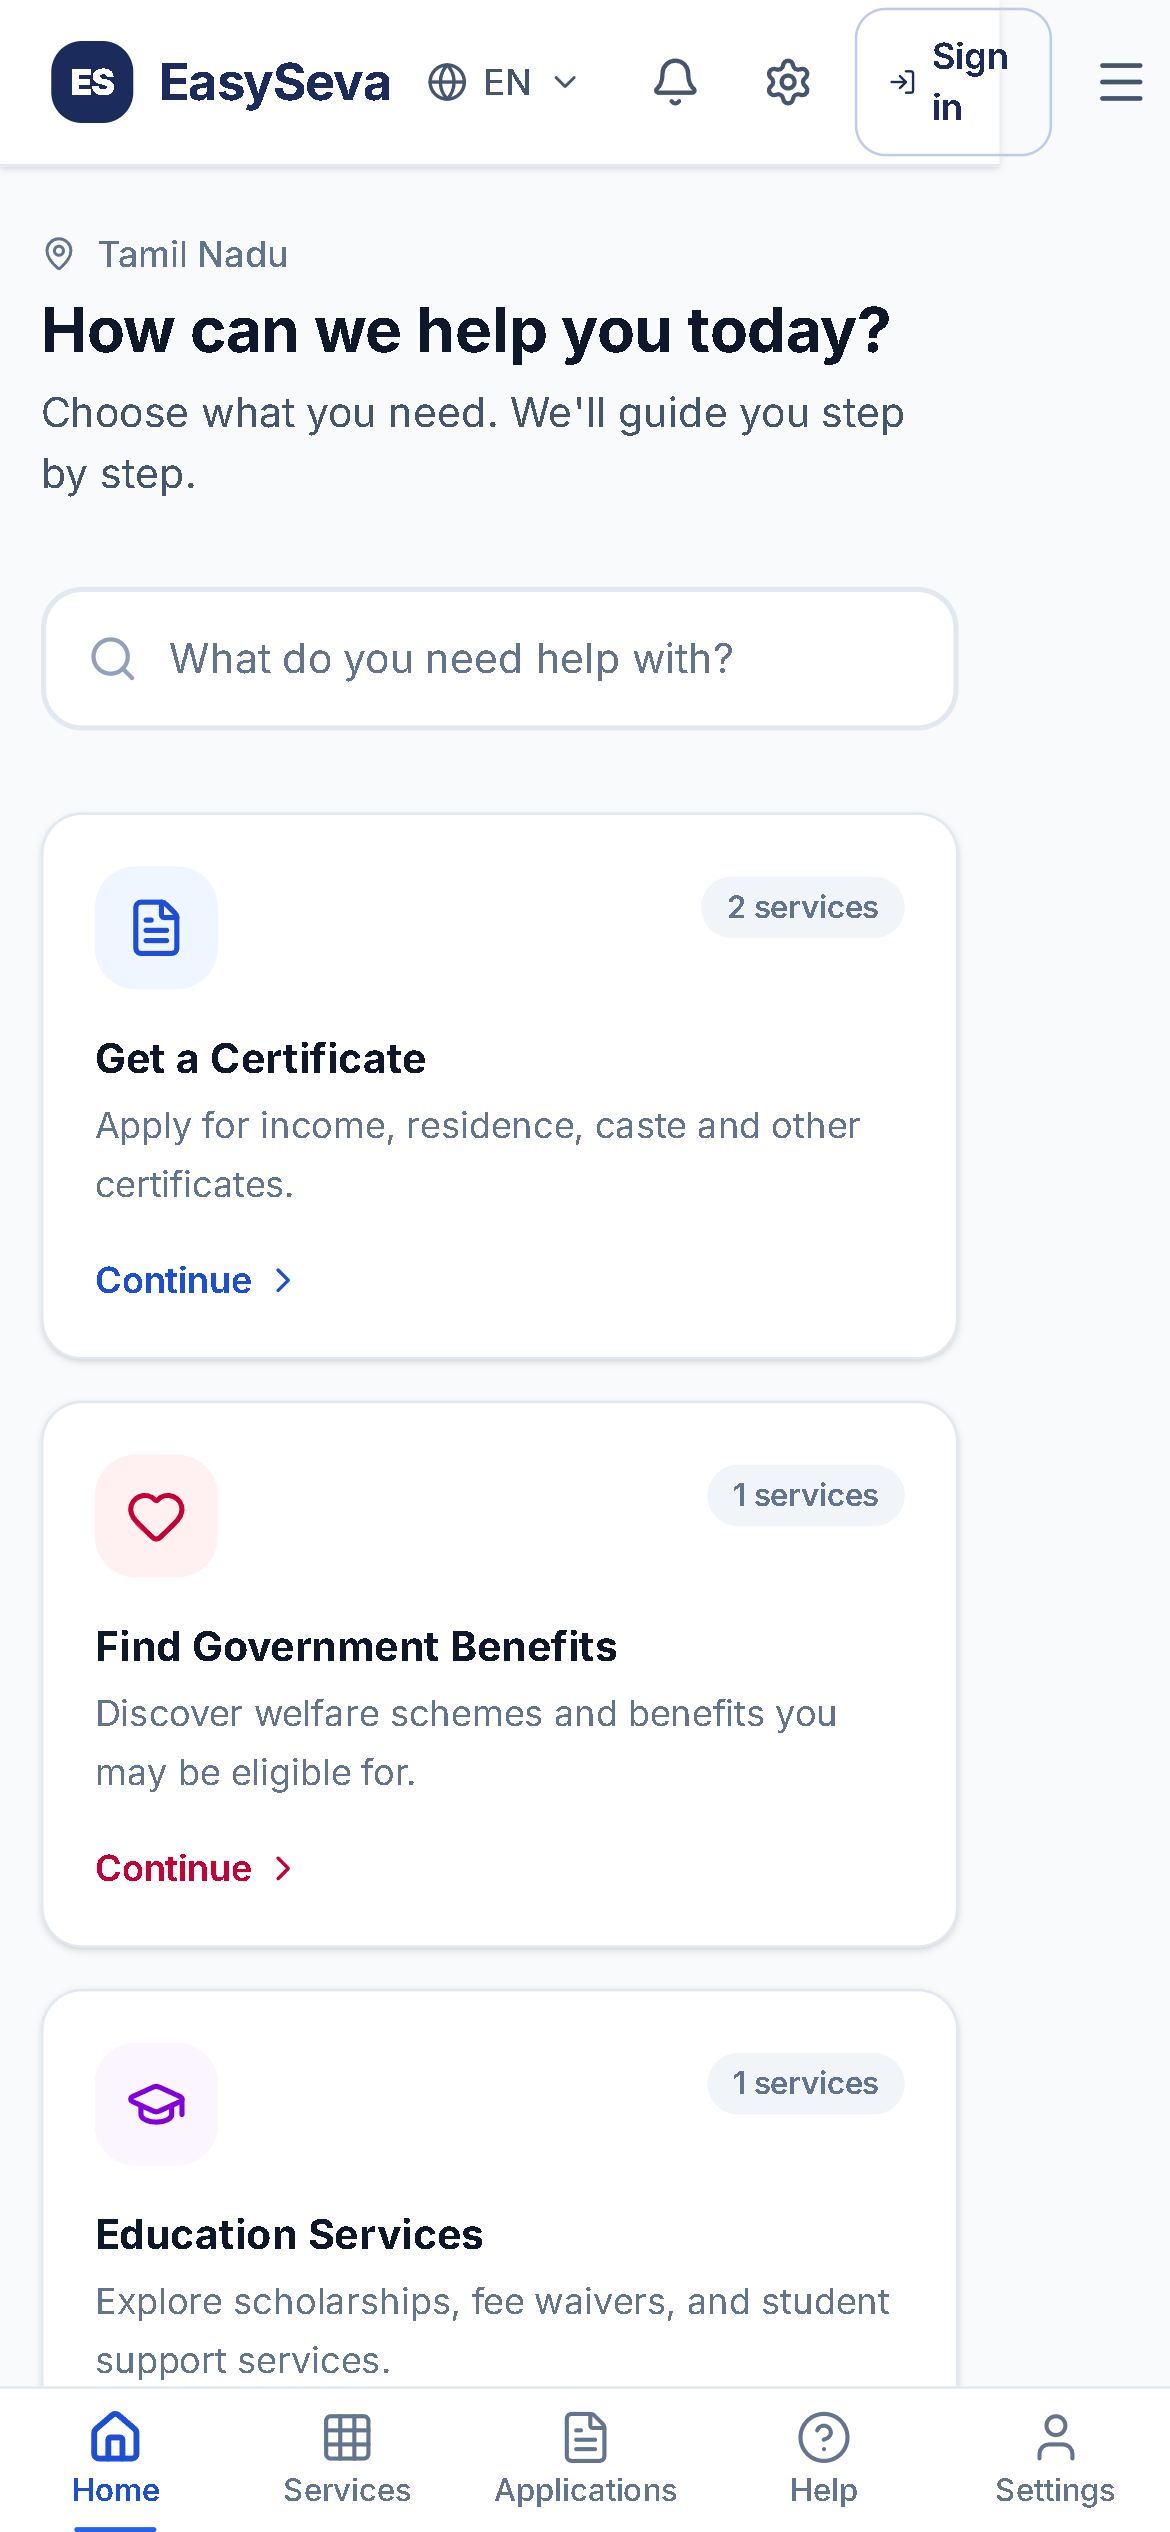
\includegraphics[height=9.5cm]{screenshots/23-mobile-home}}
\caption{The landing page and home dashboard on a phone. The layout reflows to a
single column and a bottom navigation bar appears for thumb-friendly reach.}
\end{figure}
\textbf{Purpose.} Serve the majority of citizens who access services on a phone.
\begin{itemize}
  \prin{Flexibility and efficiency (N7)}{Any device}{Layouts reflow from multi-
    column (desktop) to single-column (mobile) without loss of function.}
  \prin{Cater to universal usability (S2)}{Reach and touch}{A bottom navigation
    bar and large (44 px+) touch targets suit one-handed thumb use.}
  \prin{Consistency and standards (N4, S1)}{Same mental model}{The mobile and
    desktop experiences share components and language, so skills transfer.}
\end{itemize}

% ====================== CROSS-CUTTING ======================
\section{Cross-Cutting Principles}
Some principles are not tied to a single screen but are woven throughout.
\begin{itemize}
  \prin{Help users recognise, diagnose, and recover from errors (N9)}{Plain,
    constructive errors}{Error messages everywhere are human-readable and suggest
    a next step --- e.g., ``Please enter a valid 10-digit mobile number,'' or an
    OTP error that clears the field and invites a retry. Network failures fall
    back gracefully so the user is never stuck.}
  \prin{Keep users in control (S7, N3)}{Predictability}{Actions are initiated by
    the user; destructive or irreversible actions (submit) require explicit
    confirmation and can be approached via a reversible draft.}
  \prin{Consistency (N4, S1, D5)}{One design language}{Shared primitives and
    tokens make every button, card, badge, and field behave identically across
    the app.}
  \prin{Accessibility / POUR}{Inclusive by default}{Keyboard operability with
    visible focus, a skip link, ARIA roles and labels, scalable text, a high-
    contrast theme, and reduced-motion support make the app usable by a far wider
    range of people.}
  \prin{Conceptual model (D6)}{A clear mental picture}{The consistent five-stage
    journey --- discover, check, prepare, fill, confirm --- gives users an
    accurate model of ``how applying works,'' which transfers across all nine
    services.}
\end{itemize}

% ====================== MATRIX ======================
\section{Heuristic Coverage Matrix}
Table~\ref{tab:matrix} maps each Nielsen heuristic to representative places where
it is applied in EasySeva.

\begin{longtable}{p{5.3cm} p{9.2cm}}
\caption{Where each usability heuristic is applied.}\label{tab:matrix}\\
\toprule
\textbf{Heuristic} & \textbf{Representative use in EasySeva} \\
\midrule
\endfirsthead
\toprule
\textbf{Heuristic} & \textbf{Representative use in EasySeva} \\
\midrule
\endhead
\bottomrule
\endfoot
Visibility of system status & Progress bars, step indicators, status badges and timeline, loading/saving/verifying states, confirmation with reference number. \\
Match with the real world & Task-based categories, plain-language labels and statuses, worked examples, rupee formatting. \\
User control and freedom & Back links and breadcrumbs, ``Save \& Finish Later,'' editable review, cancellable confirmation dialog, ``Continue Anyway'' on eligibility. \\
Consistency and standards & Shared Button/Card/Badge/Input primitives and design tokens across every page. \\
Error prevention & Eligibility pre-check, inline field validation, document type/size checks, confirmation before submit, OTP instead of passwords. \\
Recognition rather than recall & Document examples, review summary, breadcrumbs, visible service cards, unread cues. \\
Flexibility and efficiency & Three languages, search and guided finder, OTP paste, tracking without login, keyboard navigation. \\
Aesthetic and minimalist design & One primary action per screen, chunked catalogue and forms, uncluttered hero. \\
Recover from errors & Human-readable messages with next steps, OTP clear-and-retry, graceful network fallbacks. \\
Help and documentation & Service FAQs, Help centre, ``Why are we asking this?'' and ``What can I use?'' disclosures. \\
\end{longtable}

% ====================== CONCLUSION ======================
\section{Conclusion}
EasySeva demonstrates that the difference between an intimidating government
portal and an empowering one is, largely, \emph{applied HCI}. By grounding every
screen in well-established principles --- keeping status visible, speaking the
user's language, preventing errors before they happen, favouring recognition over
recall, keeping the user in control, and designing for universal access --- the
application turns a once-a-year, high-anxiety task into a calm, guided, and
forgiving experience.

Crucially, these principles are not decoration: each one maps to a measurable
reduction in the real failures citizens face --- abandoned forms, rejected
documents, lost progress, and confusion over status. Good HCI, in other words, is
what lets technology actually \emph{serve} people. EasySeva is a working,
deployed illustration of that idea.

\end{document}
